% Chapter Template

\chapter{Methods} % Main chapter title
\label{ChapterX} % Change X to a consecutive number; for referencing this chapter elsewhere, use \ref{ChapterX}
%----------------------------------------------------------------------------------------
%	SECTION 1
%----------------------------------------------------------------------------------------
\section{A new approach to track intracerebral blood flow}
Widefield fluorescence imaging has a typical sampling rate of 25Hz \parencite{celotto2020analysis}. However, the dataset at hand was recorded at 100Hz. Highspeed recordings bear potentials for the analysis of neural signals beyond the frequency of neocortical slow waves. The high spatial resolution could in principle reveal patterns on a sub-millimetre-scale. New methods must be established to identify the origin of high frequency components. This is especially important because widefield fluorescence recordings are confounded with an error that results from the hemodynamic autofluorescence. The approach presented in this section indicates that high frequencies in the df/f signal relate to hemodynamic effects. Arguably high frequencies mainly stem from a signal that results from clusters of oxygenated blood which flow through intracerebral blood vessels of various size.\\
\begin{figure}[!htb]
\centering
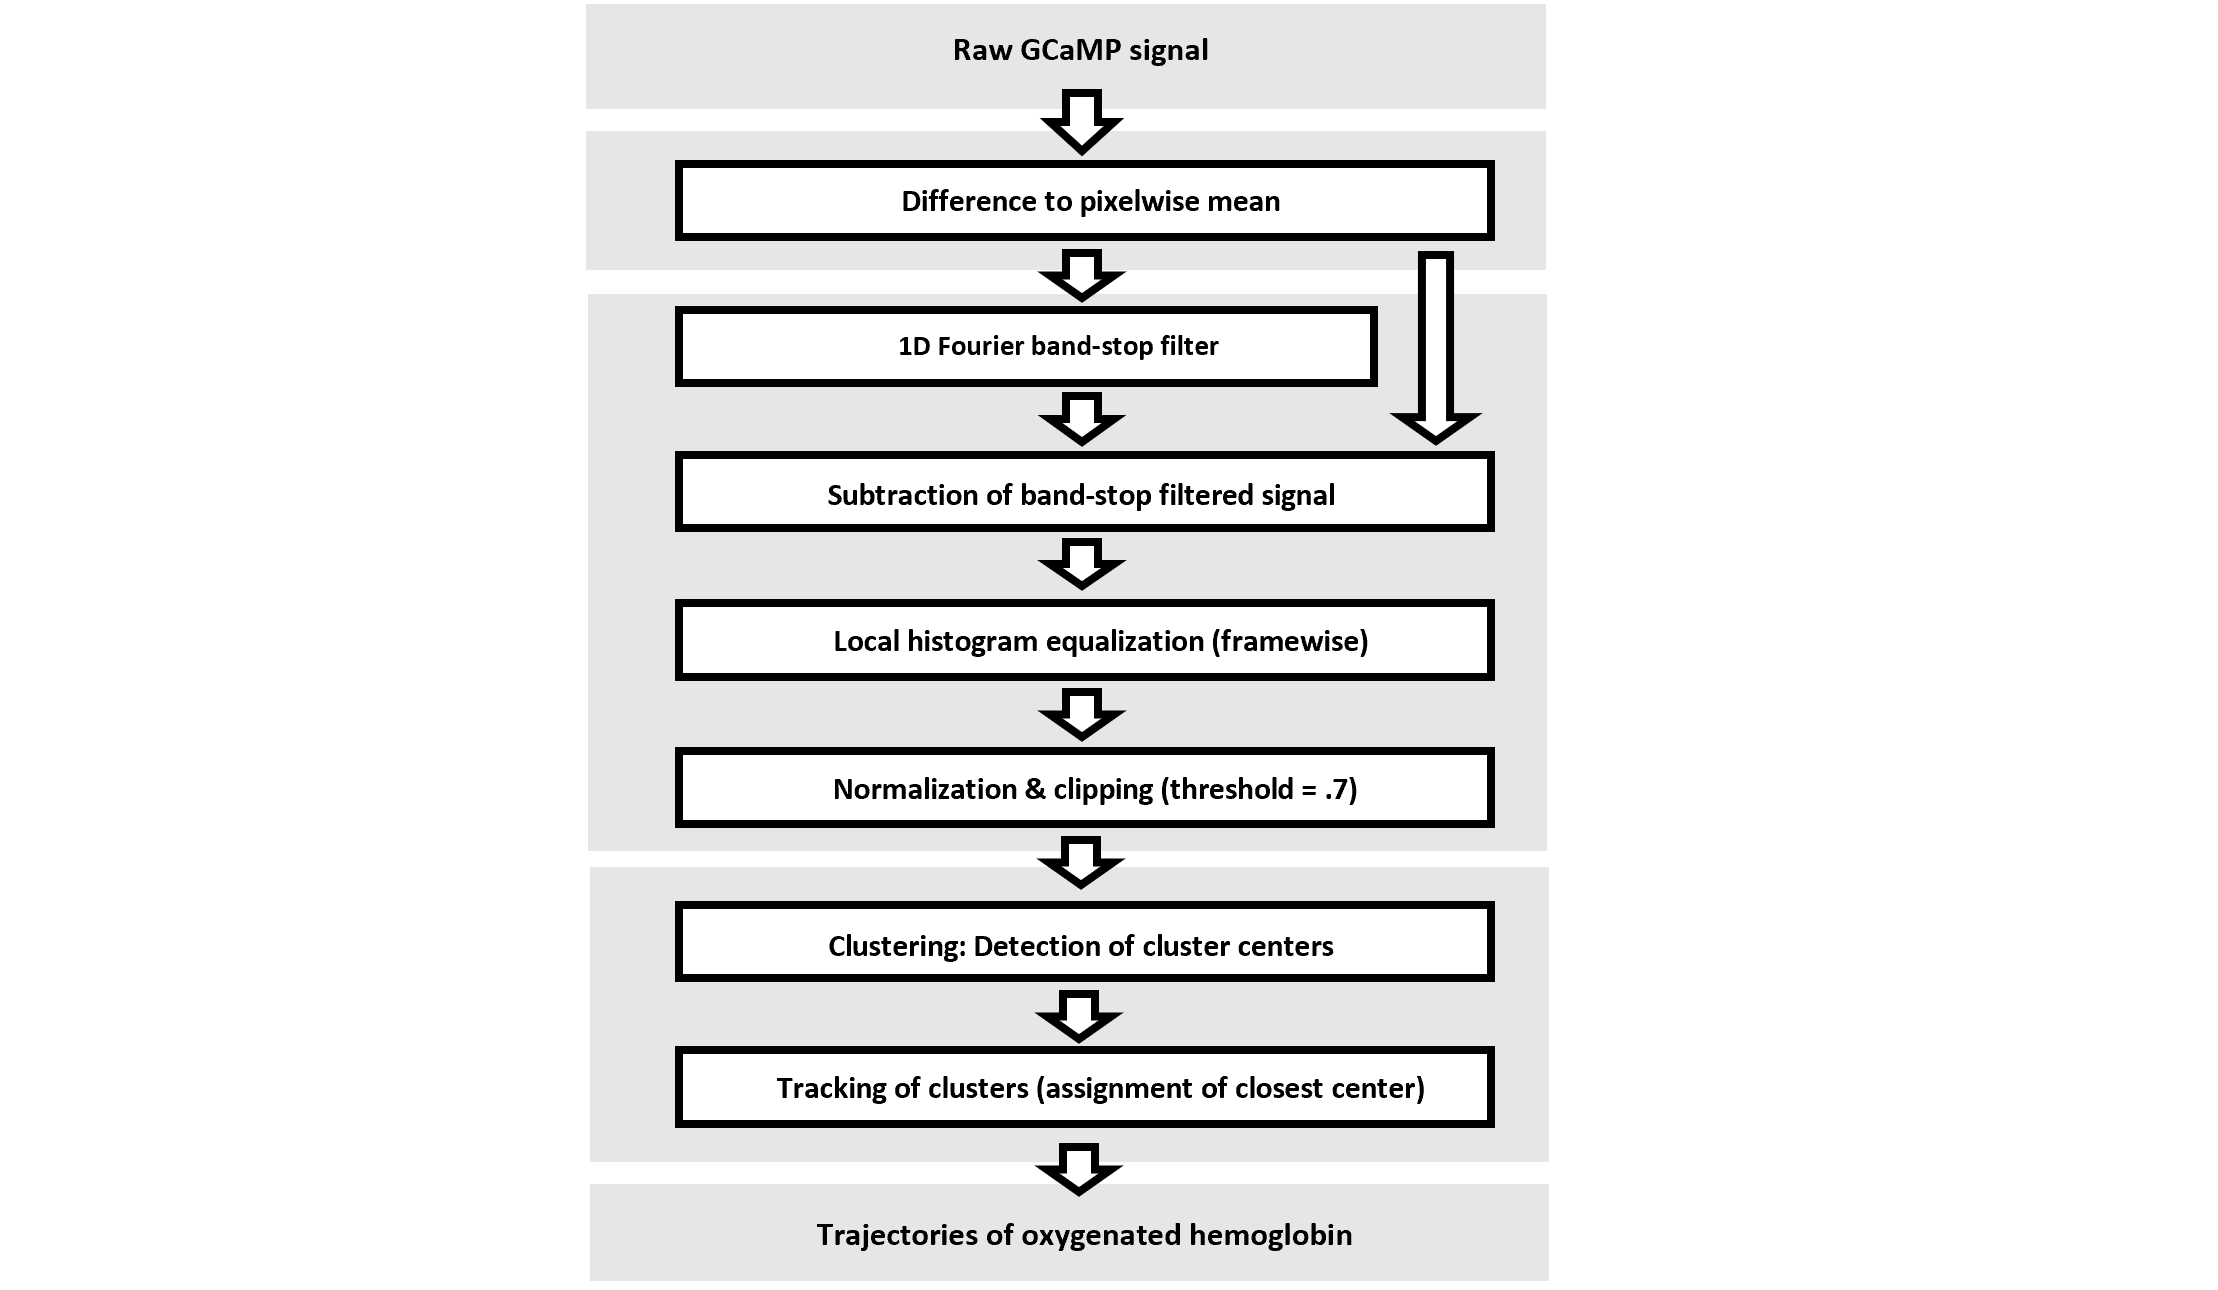
\includegraphics[width=\textwidth,height=\textheight,keepaspectratio]{Figures/tracking_bloodflow_pipeline}
\decoRule
\caption[Processing pipeline for the detection of bloodflow]{Processing pipeline for the detection of bloodflow}
\label{fig:clustering_approach_pipeline}
\end{figure}
\begin{figure}[!htb]
\centering
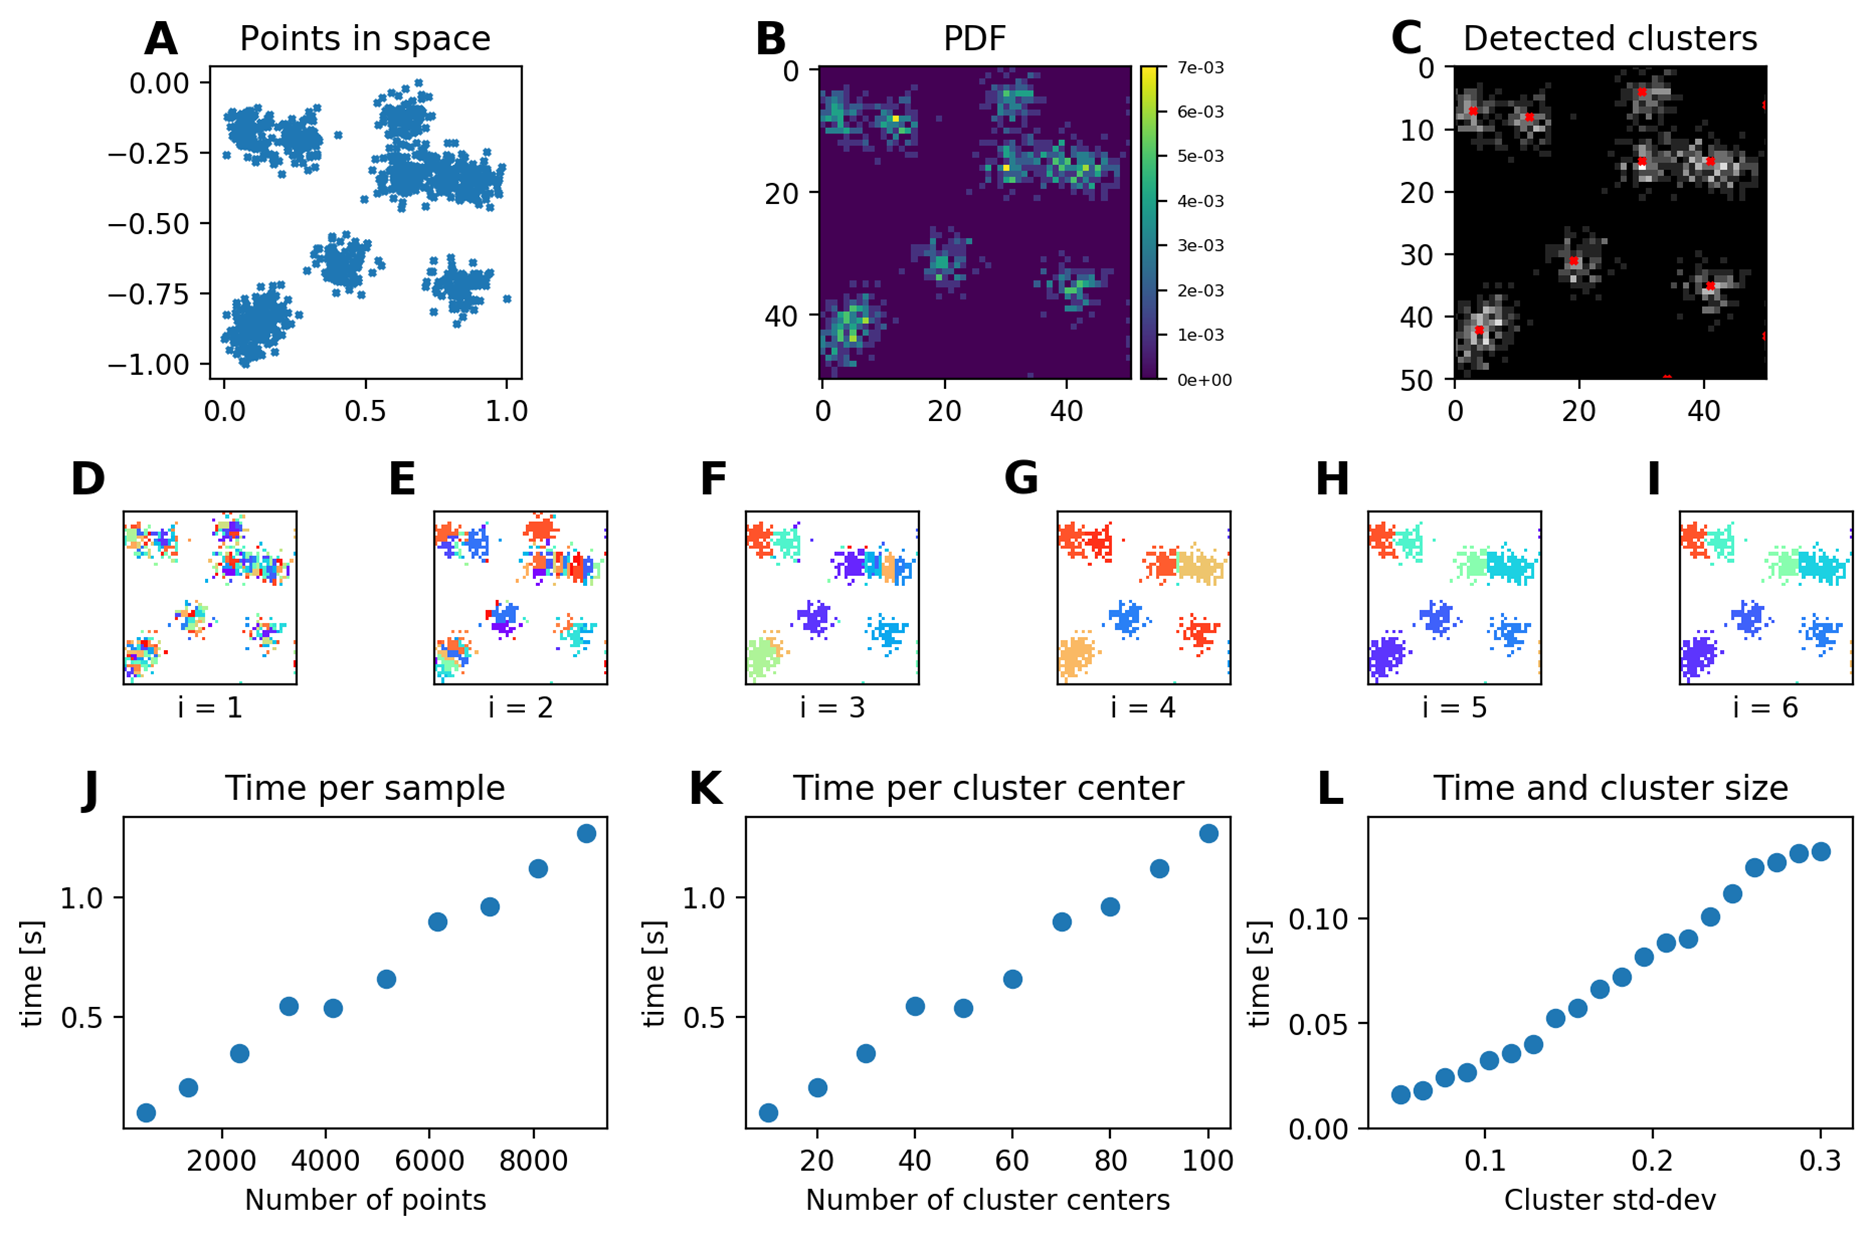
\includegraphics[width=\textwidth,height=\textheight,keepaspectratio]{Figures/clustering_approach_properties}
\decoRule
\caption[A mean shift approach for clustering pixels]{A mean shift approach for clustering pixels. After clipping the pre-processed hemodynamic signal, groups of bright, rather isolated foreground pixels are visible. These pixels can be considered as evidence for the presence of oxygenated haemoglobin particles. To detect the location of named clusters of pixels a variation of mean shift clustering was implemented that works with density matrices. Panel A: A distribution of points in $\mathbb{R^2}$. Cluster centers were sampled using a 2D gaussian. For each cluster centre points were added using a second gaussian probability distribution cantered at the respective location. Panel B : A 2D histogram of the distribution in panel A indicating the probability density function. Panel C: The detected cluster centres. Panels D-E: Assignment of pixels to clusters for the first seven iterations beginning with i=1. After iteration seven convergence is achieved. Panel J: Time per sample. Panel K: Time per cluster Panel L: Time per cluster size. }
\label{fig:clustering_approach_properties}
\end{figure}
\begin{figure}[!htb]
\centering
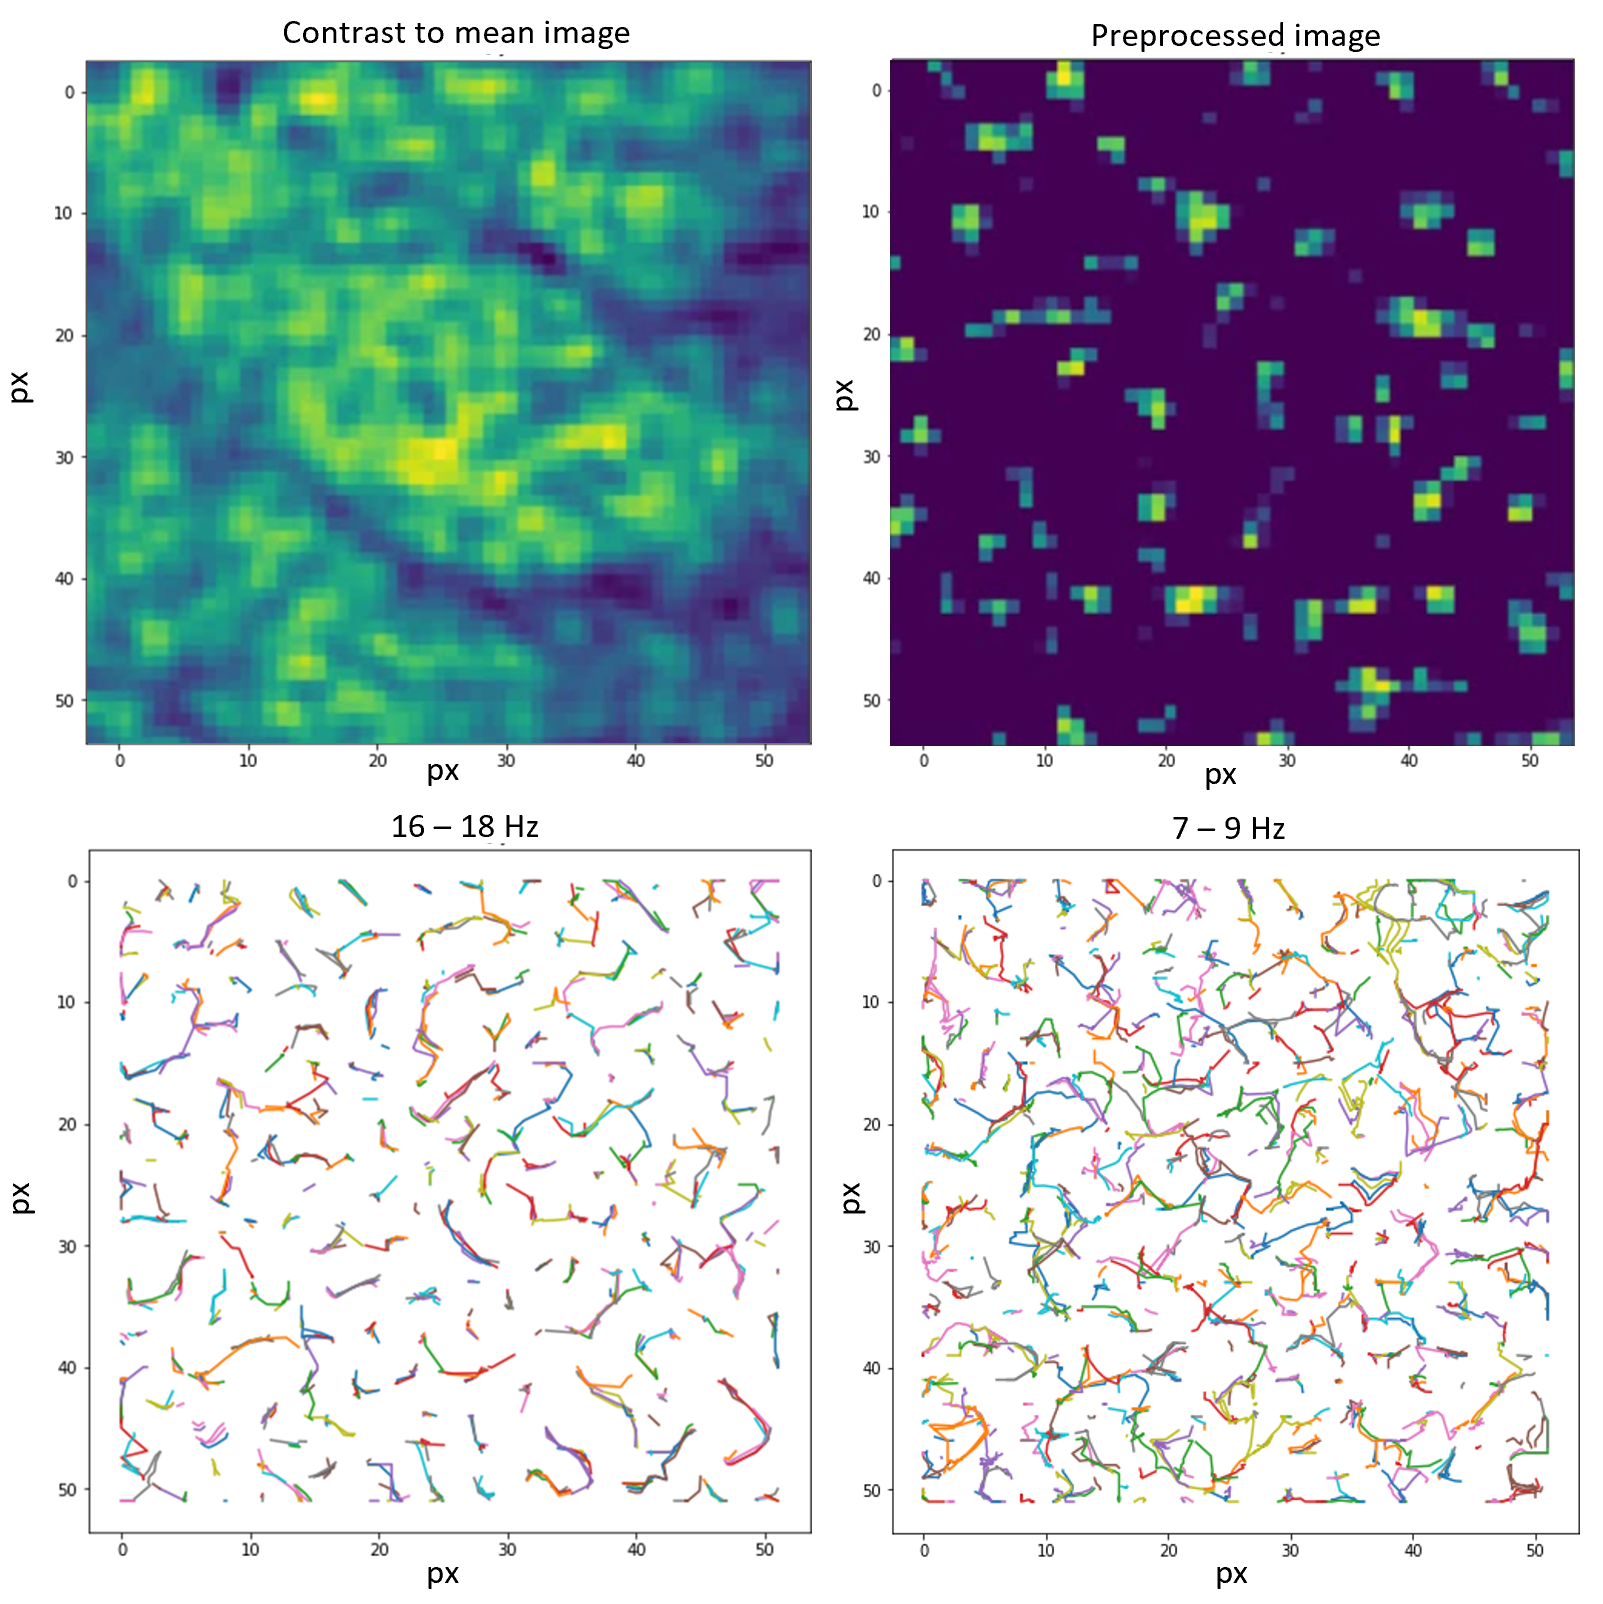
\includegraphics[width=\textwidth,height=\textheight,keepaspectratio]{Figures/clustering_approach_results}
\decoRule
\caption[Cluster tracking reveals trajectories of oxygenated hemoglobin]{Cluster tracking reveals trajectories of oxygenated hemoglobin.\\
Upper left: A sample frame for the original contrast to the pixelwise mean. Upper right: The pre-processed frame after application of clipping. Lower left: Detected trajectories for filtering of frequencies in the range of the heartbeat. Lower right: Detected trajectories of bloodflow for filtering of low frequencies. See also Figure \ref{fig:clustering_approach_properties}}
\label{fig:clustering_approach_results}
\end{figure}
The approach presented here allows to measure intracerebral blood flow without the need for the injection of tracers. Typically, microbeads are used to detect the flow rates and speed of intracerebral blood \parencite{kim2019development}. The study of intracranial blood flow bears potentials for a better understanding of pathologic conditions and basic neurobiological functions of the brain. For example, it was shown that the micro vessel density decreases in brain tumours and characteristic changes in the haemoglobin concentration can be observed in mutated tissue \parencite{lee2014vivo}. However intracerebral blood flow is also addressed in by neuroscientists in the study of neurometabolic and neurovascular coupling \parencite{devor2012frontiers}. The circumstance that the blood oxygen level dependant (BOLD) contrast is extensively used in the study of the human brain fMRI further highlights the relevance of neurometabolic effects. New approaches to track the blood flow in the brain could help to better understand the interaction between the activity of neurons and hemodynamics.\\
Several processing steps were employed to determine what high frequency components of the fluorescence signal relate to (see \ref{fig:clustering_approach_pipeline}). First the mean image was calculated and subtracted from each frame of the recorded videos. The signal in time was then band stop filtered and the difference to the original signal was calculated. Band stop filtering was achieved using 1D Fourier Transform. The signal in time for each pixel is (1) transformed to the Fourier domain (2) the frequency components in the desired range are set to zero and (3) inverse Fourier transform is applied. Adaptive histogram equalization was used to improve the contrast of each frame after clipping the values below a given threshold. In the resulting videos clusters of bright foreground pixels move on decisive trajectories (see Figure \ref{fig:clustering_approach_results}).\\
Cluster tracking is used to measure the pathways of these temporospatial patterns. Objects in binary images that are potentially connected are often labelled using watershed distance transform \parencite{arganda-carreras2016distance} \footnote{Distance transform assigns the value to the closest background pixel to each foreground pixel. Different algorithms exist that allow for fast approximations. The resulting image represents a heightmap if the distance values are interpreted as depth. A simple flooding algorithm can be used to determine the watersheds: A simulated rise of the water level fills basins in the heightmap. The borders between adjacent basins are the watersheds that separate the detected objects.}. As the data (1) was not binarized but clipped and (2) it has a low relative resolution which results in a rough outline of foreground pixels that does not allow for the computation of meaningful watersheds a different approach was used. The aim is to detect clusters of nearby foreground pixels. \\
The clipped images were interpreted as probability density functions that indicate the presence of oxygenated haemoglobin. Clusters are detected using this 2D array as the input. Each nonzero value is added to the position in an output array that corresponds to the centre of gravity of a neighbourhood around the respective pixel in the input. This procedure is repeated iteratively using the output array as the input. The centre of gravity relates to the weighted mean of the pixel coordinates along each axis where the density values are used as weights. Areas that converge to a common target location are assumed to relate to the same cluster. It is kept track of the original pixels such that the image can be labelled accordingly. The cluster centres are determined as the centre of gravity of each group. The algorithm stops if convergence is achieved or a maximal number of iterations reached. The environment for the computation of the centre of gravity could be a square or a circular patch. To reduce the impact of distant points on the centre of gravity they can be weighted using a 2D gaussian. For the results shown in Figure \ref{fig:clustering_approach_results} a simple rectangular patch was used. As the data is shifted towards the centre of gravity the approach can be considered a mean shift technique. \\
Important properties were studied stochastically using simulated data. First cluster centres were sampled from a uniform distribution. Second data for each cluster centre was sampled from a second 2D gaussian function. A smaller standard deviation was chosen for the latter function such that distinct clusters form. Note however, that an overlap was not prevented. However, it was aimed for a sparse coverage of the resulting space to limit interaction effects due to overlapping neighbourhoods of pixels from neighbouring clusters.\\
Figure \ref{fig:clustering_approach_properties} summarizes the results. The computation of 2D histograms can be achieved in O(n) as iterating over the data once is sufficient. As the size of this histogram can be chosen freely the computation time does not directly depend on the number of samples. Given that the algorithm converges, and clusters are far enough apart for the clusters to collapse independently (i.e. the neighbourhoods around the respective pixels of two neighbouring clusters never overlap) it can hence be assumed that it takes the same amount of time for each cluster in average. Hence a linear relationship between the number of clusters and the runtime can be assumed. The simulation confirmed a this assumption (see \ref{fig:clustering_approach_properties}K). Consequently, the number of samples also scales linearly with the processing time for the given sampling strategy. One may hence assume that the runtime scales linearly with the number of samples if they are arranged in small clusters with large spacings and the size of the neighbourhood is chosen accordingly. In this case the time complexity is O(n).\\
Clustering is performed for each frame separately. The result is a list of cluster centres per frame. Tracking is achieved by assigning the closest cluster centre of the subsequent frame if the maximal distance is less than ten pixels. In principle other rules can be implemented. For example, the cluster size could be considered and only those clusters can be matched that are of comparable size. Alternatively, an objective function with several constraints could be defined and used to determine the correspondence between clusters. A comparable method for cluster tracking that employs mean shift clustering in colour-space employs kernels instead of the abovementioned maximal distance rule \parencite{kumar2020tracking}. As the approach was not used to study slow waves the simplest rule for tracking was used to demonstrate the feasibility of the approach.\\
 It shows that particles move on decisive trajectories. These trajectories depend on the frequency used for band stop filtering. If band stop filtering is applied in the range of the heart rate shorter trajectories are detected and the clusters appeared to be larger. In contrast for higher frequencies a more filigree patterns can be observed. It can be hypothesized that these patterns relate to blood that travels at different speeds in vessels of different size. A more systematic study that compares trajectories revealed by the use of tracers could help putting these findings into perspective and test this hypothesis. Because of the presumed hemodynamic effect for high frequencies band stop filtering was used to reduce the impact of blood flow on the signal d in the main approach presented here.

%----------------------------------------------------------------------------------------
%	SECTION 1
%----------------------------------------------------------------------------------------
\section{Dense Optical Flow}

\begin{figure}[!htb]
\centering
\includegraphics[width=\textwidth,height=\textheight,keepaspectratio]{Figures/levelset_flow}
\decoRule
\caption[Levelsets and Optical Flow]{Levelsets and Dense Optical Flow\\ The results of an approach to track the outline of levelsets are plotted in the top row while Dense Optical Flow is plotted in the lower row. Note that only a subset of levelsets was used for the earlier approach. While Dense Optical Flow requires smooth inputs it detects similar yet dense vector fields. The movement of the wavefront of a slow wave can be represented as a binary sequence of frames. Dense Optical Flow captures the movement of multiple levelsets simultaneously and hence represents a more general approach.}
\label{fig:levelset_flow}
\end{figure}
Vector fields of pixelwise displacements that reflect the apparent motion between two subsequent video frames are called Optical Flow. Sparse Optical flow uses local features that are not necessarily present in every location of the images. Hence it yields sparse vector fields for which many values are undefined. In contrast Dense Optical Flow computes a motion vector for every pixel coordinate. Multiple algorithms exist that allow for the computation of sparse or Dense Optical Flow. \\
One class of algorithms is based on image gradients and uses iterative schemes to compute sparse or dense vector fields. Classical examples for algorithms that are still used today include the methods of Lucas and Kanade \parencite*{ lucas1981iterative} as well as  the approach suggested by Horn and Schuck \parencite*{ horn1981determining}. The approach by Lucas and Kanade \parencite*{ lucas1981iterative} depends on a linear approximation of the behaviour of a function $F(x)$ and $G(x) = F(x+h)$ in a local neighbourhood where h relates to a shift that is assumed to be sufficiently small. As Lucas and Kanade \parencite*{ lucas1981iterative}  illustrate for the one-dimensional case the approach is inspired by the formula for the numerical derivative $F’(x) = [G(x)-F(x)]/h$ or respectively $F’(x) = [G(x+h)-F(x)]/h$ that can be rearranged to express the shift as a function of the difference of both curves divided by the slope of the unshifted version: $h = (G(x)-F(x))/F’(x))$. This formula yields a good estimate especially for small shifts. To improve the estimate, a weighted average is computed for multiple values of x in a local neighbourhood. A weighting term is used that increases the impact of values for which the slope of $F(x)$ is approximately linear. To further improve the detected displacement vector an iterative scheme is employed. The previous estimate for the shift is used to move F accordingly and determine the shift again for $F(x+h)$. The estimate is updated by adding the new approximation to the preliminary displacement.  The two-dimensional form is largely identical to the one-dimensional case, however the weighting differs. As Lucas and Kanades \parencite*{ lucas1981iterative} method assumes a small shift between original image and shifted version and is based on spatial derivatives (i.e. the image gradient) it requires smooth data. Moreover, the estimate for the shift is undefined when the gradient within a local neighbourhood is all zero. Hence it is often used in combination with approaches to detect salient features and compute displacement vector only for these locations in order to retrieve sparse vector fields.\\
Here we compute dense vector fields of Optical Flow using the method suggested by Horn and Schuck \parencite*{horn1981determining}. To a certain extent it is similar to the approach suggested by Lucas and Kanade \parencite*{ lucas1981iterative}. By that it is meant that formula used to iteratively estimate the displacement vectors includes the spatial derivatives of the image as well.  However, the term also includes the temporal derivative between the pixels of the two subsequent frames. Horn and Schuck’s method computes Optical Flow using both the image gradient and the temporal derivative. Optical Flow is the result of minimizing an objective function that represents an energy functional. In analogy to the approach by Lucas and Kanade \parencite*{ lucas1981iterative} an iterative scheme can be derived. \\
\begin{equation}
  d^{k=0} = \frac{I_t}{\alpha^2+I_x^2+I_y^2}
\label{eqn:d_at_it_zero}
\end{equation}

\begin{equation}
  \begin{array}{l}
    u^{k=0}= - I_x d \\
    v^{k=0}= - I_y d
  \end{array}
\label{eqn:iterative_scheme_at_it_zero}
\end{equation}
The general form of the iterative scheme that is employed by the Horn and Schuck method is expressed by equation \ref{eqn:iterative_scheme} and \ref{eqn:d_at_it_greater_zero}. The arrays of vector components U and V are initialized with zero. Hence the general form of the iterative scheme used by the Horn and Schunck algorithm reduces to equation \ref{eqn:d_at_it_zero} and \ref{eqn:iterative_scheme_at_it_zero} for the first iteration. Two special cases can be distinguished.\\
If the temporal gradient is zero, the denominator and term d itself become zero. This means that also the vector components U and V are zero as d is multiplied with the image gradient and U and V are initialized to zero. This meets the intuition of Optical Flow. If a patch of brightness values is not shifted to a new location, there is no change in the intensity over time. Hence there is no apparent motion if the temporal derivative is zero.\\
In contrast, if the spatial gradient approaches zero the impact of a temporal brightness change on the estimated vector magnitude becomes greater. This is because the squared spatial derivatives are added in the denominator of d. Hence it scales inversely with an increasing spatial gradient. The estimate for U and V linearly depend on d. It holds that $\lim_{{I_x, I_y}\to\infty} d = I_t/\alpha $. Typically a small value is used for alpha (here 0.04). If the brightness increases by a fixed value between pairs of images that either both have a soft gradient or a steep gradient the estimated Optical Flow will be different. This meets the intuition. In the case of a soft gradient differences in brightness between far apart areas are small. Hence, a small increase in brightness is sufficient to displace areas with a given grey value over large distances. Intuitively gradient based methods for Dense Optical Flow can be interpreted to indicate the displacement of grey values.\\
\begin{equation}
  d = \frac{(I_x\overline{u}^k+I_y\overline{v}^k+I_t)}{\alpha^2+I_x^2+I_y^2}
\label{eqn:d_at_it_greater_zero}
\end{equation}

\begin{equation}
  \begin{array}{l}
    u^{k+1}=\overline{u}^k - I_x d \\
    v^{k+1}=\overline{v}^k - I_y d
  \end{array}
\label{eqn:iterative_scheme}
\end{equation}
Besides classical approaches there are many other techniques that allow for the computation of Optical Flow \footnote{For a comparative evaluation on the Sintel dataset see Max Planck Institute \parencite*{mpi2020sintel}}. These approaches are not necessarily based on gradients. Co-registration of patterns can for example also be achieved by retrieval and matching of scale invariant features \parencite{zhang2014scale}. More recently deep neural networks have been proposed. Networks that employ regression layers and are trained in an end-to-end fashion to predict dense vector fields. While it was noted that domain specific overfitting must be addressed, they have been demonstrated to outperform other approaches for videos that depict natural scenes. The task of direct prediction of displacement vectors is typically addressed using Autoencoders for the transfer from the image domain to motion fields \parencite{hur2020optical}. Dense Optical Flow can be understood a nonlinear mapping from dense pixel arrays to vector fields. \\
In neuroimaging the spread of slow waves is typically measured using delay maps \parencite{celotto2020analysis}. Local minima can be detected that indicate whether an event as already started for a point in time for a given discrete time interval. The result can be displayed as a binary video where the transition from positive to negative values reflects the position of the wavefront. Here it was aimed for a description of slow waves that can potentially incorporate several oscillations that may occur simultaneously and even overlap. Hence an approach was tested that can handle both binary wavefronts and level set flow. \\
The relationship between moving wavefronts and Optical Flow can be demonstrated using an approach that allows to track level sets. Level Set Flow computes displacement vectors for binary level sets. A vector field is computed in which vectors point towards the outline of the binary object. This is achieved by the computation of Distance Transform of the foreground and the background pixels of the target frame. The results are stored in a single 2D array. This representation can be interpreted as a scalar potential. The outline of the foreground pixels is detected in the source image. Then gradient descent is performed beginning at each of the coordinates of named pixels following the gradient of the scalar potential. Once a position is reached where the target matrix is false the procedure stops and is repeated for the next coordinate. The approach yields vectors that indicate the displacement of the outline of binary level sets.\\
It shows that Horn and Schuck’s method for Optical Flow computes vector fields that resemble the movement of level sets. However sufficient smoothing is required. The method of Horn and Schunck \parencite*{ horn1981determining} has already been demonstrated to be useful for the characterization of temporo-spatial-patterns in fluorescence recordings \parencite{townsend2018detection}. Neuroimaging data represents non-textured data, can satisfy the smoothness requirements and hence be used for the computation of Dense Optical Flow using Horn and Schucks method. Dense vector fields are required for the application of Helmholtz Decomposition.
\section{Helmholtz Decomposition}
Vector fields can be used to describe various physical phenomena including fluid dynamics or magnetic flux but also the dynamics of spreading waves of neural activity. Dense vector fields of displacements can be computed from fluorescence recordings using Dense Optical Flow \parencite{townsend2018detection}. Patterns in these vector fields can be used to characterize the way neural signals travel in cortex during slow wave sleep and anaesthesia. Townsend and Gong \parencite*{townsend2018detection} suggest a kernel-based approach to detect several local and global features. A more general approach that allows to study fundamental properties of vector fields is Helmholtz Decomposition. \\
Smooth vector fields can exhibit a complex structure that can be described in several ways. There are properties such as the field strength that can be computed for every vector individually. Besides a distinction can be made between local patterns that relate to a subset of neighbouring vectors and global features that describe the vector field as a whole. Local patterns include inward spirals or patches of vectors that point towards a specific location or line surrounded by them. Townsend and Gong \parencite*{townsend2018detection} describe the latter two examples as stable nodes and saddles. In contrast unstable nodes and outward spirals relate to patterns where vectors point away from a secific location. An example for a feature that decribes the vector field as a whole are plane waves in velocity fields that describe the average normalized speed \parencite{townsend2018detection}. These patterns may occur in isolation, but they can also co-occur and create complex structures of potentially overlapping features. For example spirals can be expressed as an addition of a diverging vector field and one with nonzero curl \parencite{cedmav2020natural}. This raises the question what the fundamental components of vector fields and their characteristic properties are.\\
\begin{equation}
  \text{div } \vec{F} = \frac{\partial P}{\partial x} + \frac{\partial Q}{\partial y}
\label{eqn:divergence}
\end{equation}
\begin{equation}
  \text{curl } \vec{F} = \frac{\partial Q}{\partial x} - \frac{\partial P}{\partial y}
\label{eqn:curl}
\end{equation}
Two important local properties of vector fields are curl and divergence. "Divergence is an operation on a vector field that tells us how the field behaves toward or away from a point" \parencite{strang2018divergence}. Areas where a vector field contains sources or sinks have nonzero divergence. To compute divergence for a 2D vector field (1) the numerical derivative of the 2D array of X components is retrieved along the X axis, (2) the numerical derivative of the respective array of Y components is computed along the Y axis and (3) the resulting 2D scalar arrays are added. In other words divergence relates to the sum of the partial derivatives of the vector components with respect to the vector dimension they express (Equation \ref{eqn:divergence}). The computation of curl is based on partial derivatives of the vector components as well. However, curl is defined as the difference between the partial derivative of the Y-components (Q) with respect to X and the partial derivative of the X-components (P) with respect to Y (Equation \ref{eqn:curl}). An example for a vector field that has nonzero curl is F(x,y)=[y,-x]. It shows circular flow and has zero divergence.\\
\begin{figure}[!htb]
\centering
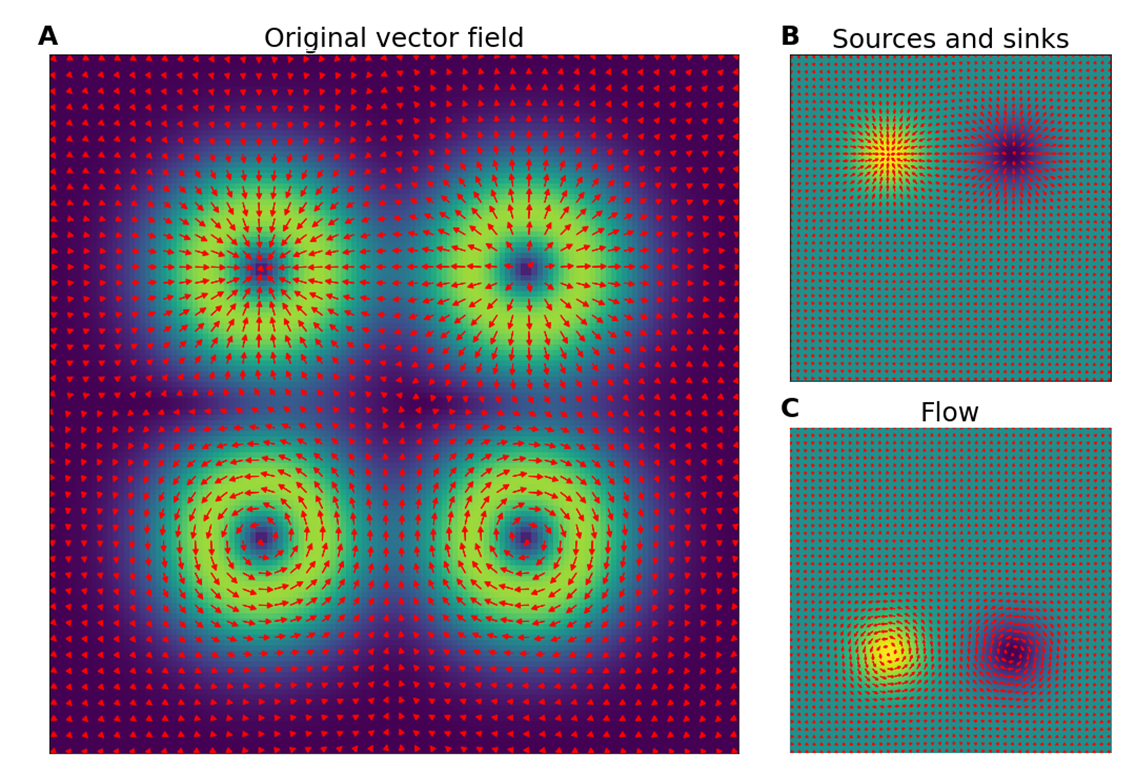
\includegraphics[width=\textwidth,height=\textheight,keepaspectratio]{Figures/helmholtz_decomposition}
\decoRule
\caption[Helmholtz decomposition of a sample vector field]{Helmholtz decomposition of a sample vector field.\\ Panel A: A vector field that contains a sink (top left), a source (top right) as well as areas with positive and negative curl (bottom left and bottom right). The field strength is plotted in the background. Panel B: The distribution of sources and sinks. The scalar potential of the curl free component is plotted in the background. Note that yellow tones indicate posive values while blue tones indicate negative values. The gradient field is plotted in the foreground. Panel C: The flow component. The scalar field is plotted in the background where blue tones relate to negative and yellow tones to positive values. The vector field $mathrm{\nabla}\varphi_{div=0}$ is plotted in the foreground.}
\label{fig:helmholtz_decomposition}
\end{figure}
Helmholtz Decomposition allows to decompose vector fields into a curl free and a divergence free component. It is used in several disciplines to study various phenomena. Helmholtz-Decomposition can be used to model weather phenomena, ocean currents, electromagnetism, geophysical phenomena but it is also used in computer graphics and computer vision \parencite{bhatia2012helmholtz}. Applications in neuroimaging exist as well. Helmholtz Decomposition has been used in combination with Dense Optical Flow of heightmaps that indicate cortical growth captured by MRI to determine growth seeds in the neonate brain \parencite{lefevre2009identification}. \\
 The fundamental theorem of vector calculus (Helmholtz-Theorem) states that every vector field can be expressed as the sum of a curl free and a divergence free vector field if it is sufficiently smooth and decays rapidly. The definition is given by Equation \ref{eqn:helmholtz_decomposition}. The curl free vector field relates to the distribution of sources and sinks. In contrast the divergence free component is also referred to as flow. Helmholtz Decomposition is used to retrieve these two components for a given vector field. This is achieved by an approximation of the scalar potential of the curl free component and a scalar field for the flow. The respective vector fields are defined as $\mathrm{\nabla}\varphi_{curl=0}$ and $J\mathrm{\nabla}\varphi_{div=0}$. Sources have negative values in the scalar potential of the curl free component while sinks have positive values. In contrast areas with rightwards curl and leftwards curl have negative and positive values in the scalar field of the divergence free component. Figure \ref{fig:helmholtz_decomposition} illustrates the decomposition of a vector field that contains a source and a sink as well as areas with rightwards and leftwards curl in distinct areas.\\
\begin{equation}
  v=\mathrm{\nabla}\varphi_{curl=0}+J\mathrm{\nabla}\varphi_{div=0}
\label{eqn:helmholtz_decomposition}
\end{equation}
 There are several ways to compute Helmholtz Decomposition. Most approaches are based on the minimization of an energy functional. However, Machine Learning can also be employed to compute the divergence free component and the curl free component. For example a radial basis function (RBF) can be trained to learn the mapping between a vector field and the curl free or the divergence free component. Named approach employs statistical learning and is suitable for potentially noisy data \parencite{bhatia2012helmholtz}. Here natural Helmholtz Decomposition is used to decompose vector fields of Dense Optical Flow and retrive the curl free component as well as the divergence free component \parencite{bhatia2014natural}. \\
\begin{figure}[!htb]
\centering
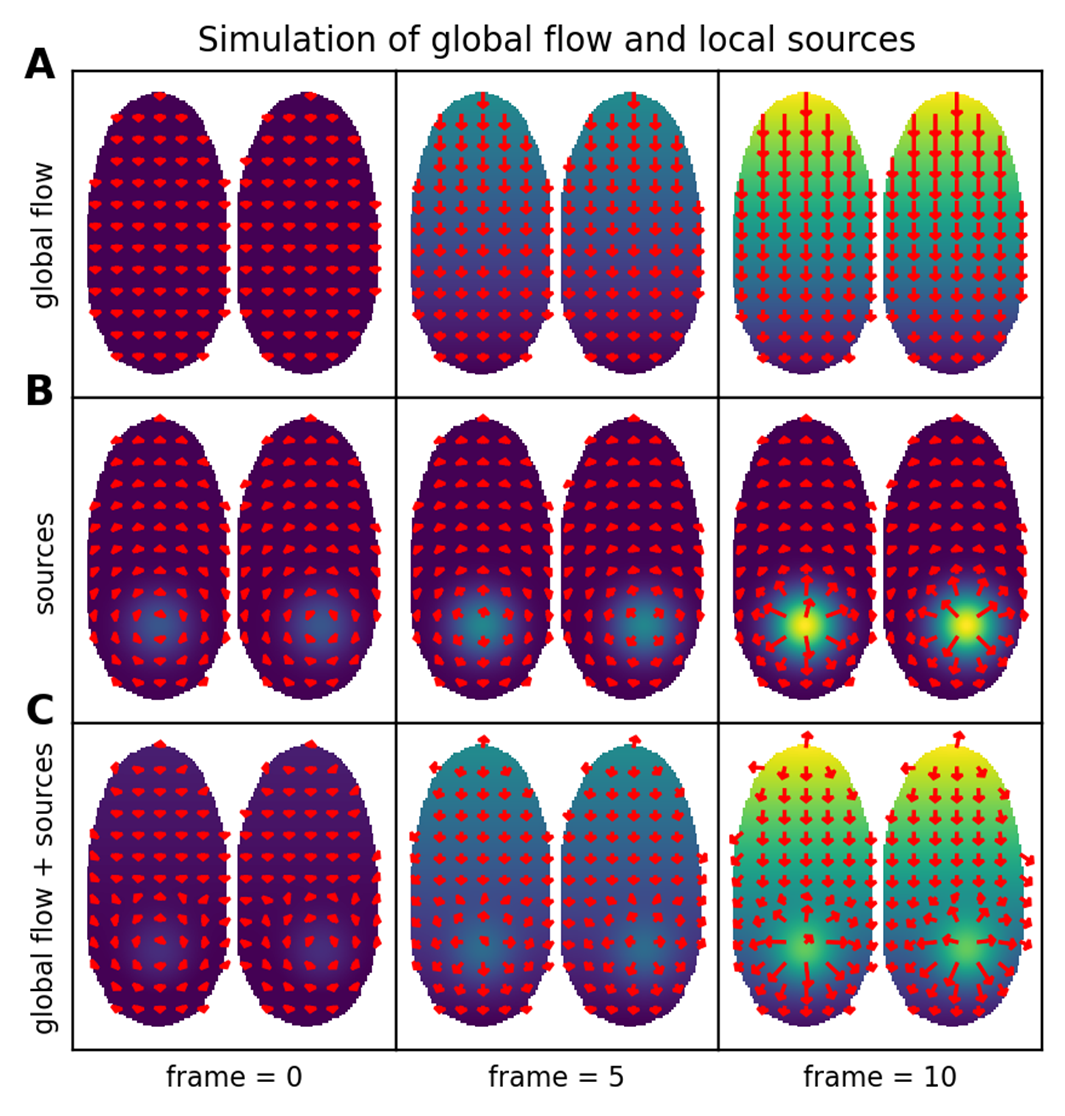
\includegraphics[width=\textwidth,height=\textheight,keepaspectratio]{Figures/optical_flow_for_a_simulated_signal}
\decoRule
\caption[Optical flow for a simulated signal]{Optical flow for a simulated signal\\ Panel A (top row): Three frames from a sequence where a global brightness gradient increases in intensity. Panel B (middel row): Areas of focal brighness change and the resulting sources and sinks. Panel C (lower row): The sum of the signal in A and B. Optical flow was computed for each sequence of frames and is plotted in the foreground.}
\label{fig:optical_flow_for_a_simulated_signal}
\end{figure}
\begin{figure}[!htb]
\centering
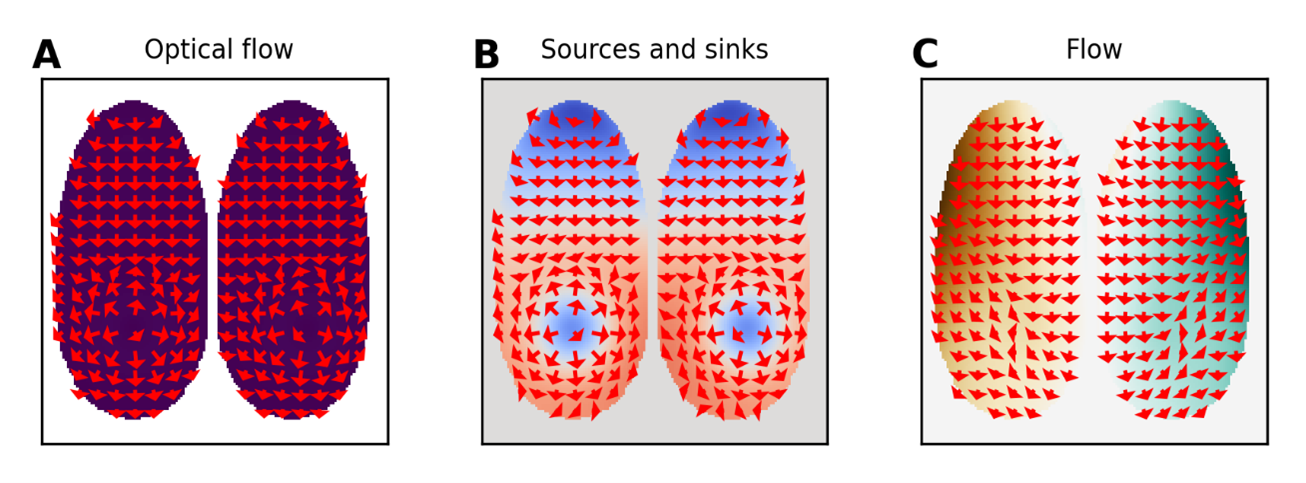
\includegraphics[width=\textwidth,height=\textheight,keepaspectratio]{Figures/helmholtz_decomposition_of_optical_flow_simulation}
\decoRule
\caption[Helmholtz Decomposition of Optical Flow]{Helmholtz Decomposition of Optical Flow.\\ Panel A: A vector field of Dense Optical Flow that contains sources and global flow. The respective brightness distribution is shown in the background (see also Figure \ref{fig:optical_flow_for_a_simulated_signal}C). Panel B: The distribution of sources and sinks retrieved using Helmholtz Decomposition of the vector field in A. The scalar potential is plotted in the background. Note that focal areas of brighness increase have positive values in the scalar potential of the curl free component. Panel C: The flow component of the vector field in A. Note that the impact of focal areas of brightness increase on the resulting flow field is highly reduced. Helmholtz-Decomposition allows to distinguish global flow from focal areas of brightness increase or decrease.}
\label{fig:helmholtz_decomposition_of_optical_flow_simulation}
\end{figure}
Helmholtz Decomposition is applied on Dense Optical Flow. To illustrate the relationship between the change in brightness in the original signal and Helmholtz Decomposition of Dense Optical Flow the approach was applied on simulated data. Two sequences of frames were computed. The first signal represents a global brightness gradient with an increase in intensity over time. The second signal was generated by gaussian smoothing of a binary 3D array where the X and Y axis relate to space and the Z axis relates to time. This 3D array was initialized with zeros and two areas that represent a cuboid were filled with a positive value. A third signal was generated by the addition of both named signals. Optical Flow was computed subsequently for each frame the three signals. The Optical Flow of the combined signal was then decomposed into the distribution of sources and sinks as well as the flow component.\\
It shows that the distribution of sources reflects focal areas of an increase in brightness. In the fluorescence recordings this local increase can be assumed to result from recurrent activity in distinct areas of the brain. In contrast the vector field of the flow component reflects the Optical Flow of the first of the three simulated signals. The impact of focal brightness changes on the vector fields can be highly reduced. The flow component can be assumed to reflect scenarios where peak activity shifts from one area to another or a global wave spreads through a hemisphere.

\section{Autoencoders}
Neuroimaging techniques allow for the aquisition of data with a high temporospatial resolution. This means that the recordings are of high dimensionality. However specific features are especially interesting: The location of focal areas of recurrent activity, the amplitude of the event and the direction of flow. Feature engineering that relies on Optical Flow and Autoencoders can be used to retrieve these features with a high degree of control. This allows to reduce the dimensionality of the data and promises robust features. Further dimension reduction can be achieved using unsupervised learning. It can be assumed that slow waves are either similar with respect to the mentioned properties or to differ substantially. Low dimensional representations can help to identify different types of slow waves. Here Autoencoders are used for dimensionality reduction as they allow for the approximation of nonlinear functions and are well suited for images.\\
Autoencoders can be understood as a more general approach to dimension reduction as compared to Principal Component Analysis (PCA). An Autoencoder with a single hidden layer, a linear activation function and a squared error cost function is almost identical to PCA: After successful training the weights span the same subspace as the Eigenvectors in PCA. However, the weights are not necessarily identical \parencite{plaut2018principal}. Both PCA and single layer, linear Autoencoders with squared error loss can be used to linearly map data onto a lower dimensional subspace\footnote{Here it is assumed the Autoencoder has fewer latent layer neurons than inputs. Note that Autoencoders could in principle also have latent layers with a higher dimensionality as the input and target layers. A typical example are sparse Autoencoders \parencite{paperswithcode2021sparse}.}.
Simple Autoencoders employ a Multilayer Perceptron (MLP) as the encoder and decoder. Here MLP is used in the strict sense and relates to feedforward networks that comprise of fully connected layers only. This form of Autoencoder was described as an alternative to PCA already when the computational power of available machines was limited \parencite{kramer1991nonlinear}. In the most simple case weights are learned using gradient descent and backpropagation to minimize the reconstruction loss only: In this case the data is used as both the input layer activation and the output layer activation. MLPs are nonlinear function approximators and hence promise better reconstructions for low dimensional latent layers as compared to linear mappings. Autoencoders represent a powerful and flexible tool for the unsupervised analysis of high dimensional data.\\
 There are numerous applications of Autoencoders in biomedical imaging and neuroscience for various domains of data. Autoencoders that employ convolutional layers are especially well-suited for images. For example Autoencoders can be used to detect tumors in the brain or the liver using Magnetic Resonance Imaging (MRI) or Computer Tomography (CT) \parencite{mallick2019brain, sital20203d}. Similarly they can be used to label and detect brain lesions \parencite{alex2017semisupervised}. Autoencoders can also be used in combination with fMRI. For example it was shown that the visual perception of participants can be decoded from fMRI recordings. A variational Autoencoder (VAE) is trained on the videos that participants watched during data aquisition and a linear regression model mapping is used to map the BOLD response to the latent layer activations such that the decoder can predicts the frames \parencite{han2019variational}. Autoencoders can be used for unsupervised learning and semi-supervised learning. The latter case is especially relevant if labels exist for a subset of the dataset. Besides there are several ways in which Autoencoders can be used aiming for potentially different objectives. Multiple examples exist:\\
\begin{enumerate}[label={(\arabic*)}]
    \item Dimension reduction. If Autoencoders are used for dimension reduction the latent layer activation is of interest. The same data that is used for the input layer is predicted by the output layer \parencite{han2019variational}.
    \item Artifact removal and denoising. If Autoencoders are used for artifact removal or denoising data with artifacts is used as the input to predict an artifact free version. Denoising Autoencoders are models that are trained on data with added noise to avoid learning the identity function which is especially important if the bottleneck layers are of high dimensionality \parencite{paperswithcode2021denoising}
    \item Attribution of pixelwise labels. In this case source data is used which is different from the target data. A common example is semantic labelling of natural images or medical images. In this case semi-supervised learning is employed \parencite{alex2017semisupervised}.
    \item Domain transfer. An example for domain transfer is the mapping between 2D images and 3D point clouds \parencite{lin2018learning}.
    \item Semantic Image Augmentation. An example for this category is image colorization \parencite{anwar2020image}.
\end{enumerate}
Different versions of Autoencoders exist that employ a custom loss function. Besides modifications that are necessary to achieve good predictions there are loss functions that are used to shape latent space. The most well-known examples are VAEs and Autoencoders for semisupervised learning. Here VAEs are used. The loss function of a VAE contains the reconstruction loss which is added to a second term (the KL-loss), that is based on the Kullback–Leibler divergence and penalizes noncontinuous distributions of the data in latent space. The models used here were derived from standard VAEs. The activation of the latent layer $z$ depends on the resampled activity of two previous layers $z_{mean}$ and $z_{logvar}$ that connect it to the encoder and have a linear activation function. The resampling function is given by Equation \ref{eqn:resampling}. The KL-loss is given by Equation \ref{eqn:kl_loss}.\\
\begin{equation}
\text{sampling}(Z_{mean}, Z_{log var}) = Z_{mean}+ \exp(0.5 * Z_{log var}) * \mathcal{N}(\mu = 0,\,\sigma^{2}=1)
\label{eqn:resampling}
\end{equation}
\begin{equation}
  \text{KL}_{loss} = -0.5 * \sum 1 + Z_{log var} - Z_{mean}^2 - \exp(Z_{log var})
\label{eqn:kl_loss}
\end{equation}
The structure of Autoencoders depends on the objective for which they are used and has to meet the constraints of the data. Deep Autoencoders that employ strategies to overcome the vanishing gradient problem have been employed with great success to label medical data \parencite{du2020medical}. An example is UNet which uses direct links that connect early layers of the encoder and late layers of the decoder. In the moste simple version (Base UNet) links are achieved by concatenation of the output from the contracting path to inputs of layers of the expansive path. In other variations such as UNet++, additional convolutional layers are used between encoder and decoder \parencite{du2020medical}. UNet can also be used as part of a generative adversarial network. In this case a discriminator network is connected to the output of the decoder to distinguish between generated labels and training labels. Generative adversarial networks promise reconstructions with higher levels of detail. Variations of UNet have been used for tissue segmentation and cancer detection in numerous studies using MRT, MRI and ultrasound \parencite{du2020medical}. \\
  Here Autoencoders are used on relatively sparse features as only specific properties of the data are of interest and major parts of the variance are arguably not necessary to reflect them. The main purpose is dimension reduction. The possibility to assess the quality of intermediate representations and to compute meaningful aggregations could help increasing the interpretability of the results. Training on sparse features also means that comparatatively shallow networks can be used.\\
\begin{figure}[!htb]
\centering
\includegraphics[width=\textwidth,height=\textheight,keepaspectratio]{Figures/Autoencoder_1_mlp}
\decoRule
\caption[Structure of the MLP Autoencoder]{Structure of the MLP-Autoencoder.\\ This Autoencoder was used for the analysis of slow-wave-shape space. Rectified linear units (RELU) activation functions were used if not stated otherwise. The df/f signals for each detected event are normalized and interpolated to be of equal length (128 entries). The duration and amplitude of each event were appended.}
\label{fig:Autoencoder_1_mlp}
\end{figure}
Three different Autoencoders were implemented to analyse the extracted slow wave features. The first Autoencoder was used to analyse the distribution of the detected samples in slow-wave-shape-space. It showed that different events have similar signatures in the df/f signal. Hence it was aimed for a simple Autoencoder that can be used to encode relatively sparse values. A simple MLP-Autoencoder was implemented for this purpose where all layers are fully connected. As different slow waves were found to have similar shapes but differ in amplitude the df/f signal of each event was normalized and interpolated and the peak amplitude was appended. This approach was chosen such that it is possible to excert control over the impact of differences in amplitude on the reconstruction loss. The resulting structure of latent space reflects similarities in shape and size of events.\\
\begin{figure}[!htb]
\centering
\includegraphics[width=\textwidth,height=\textheight,keepaspectratio]{Figures/Autoencoder_2_mixed_input}
\decoRule
\caption[Structure of the mixed input Autoencoder]{Structure of the mixed input Autoencoder.\\ This Autoencoder was used to analyze (1) the distribution of sources and sinks (2) the df/f signal and (3) scalar values that reflect the amount of flow in upwards, downwards rightwards and leftwards direction alongside the duration and amplitude of each event. Different encoders and decoders were used for each domain of data. 2D convolution was used for encoding and decoding the distribution of sources and sinks, 1D convolution was used for the time series signal and fully connected MLP layers for the scalars. Note that different branches were introduced in the respective value decoder. This was found to help optimizing the predictions for the directions of flow and at the same time the duration and amplitude of each event. RELU activation functions were used if not stated otherwise.}
\label{fig:Autoencoder_2_mixed_input}
\end{figure}
The second Autoencoder represents a mixed input model (Figure \ref{fig:Autoencoder_2_mixed_input}). Several different features were used as the input and output activations. These features include grayscale images that represent the mean distribution of sources and sinks for each event, the normalized df/f signal, the phase and peak amplitude as well as the ratio between upwards, downwards leftwards and rightwards flow. Different modules were implemented for the encoder and decoder that were considered best suited for the respective type of data. Images and time series represent data that contains local features. Hence 2D convolution was used for the distribution of sources and sinks. In contrast 1D convolution was used for the time series. 1D convolution was realized using 2D convolution with 1XN shaped kernels. MLP layers were used for the scalar values. \\
\begin{equation}
\text{loss} = \text{KL}_{loss}(z_{mean},z_{logvar}) + \sum p_i * \text{MSE}(\text{data}_i, \text{VAE}(\text{data})_i)
\label{eqn:custom_loss}
\end{equation}
\begin{equation}
\text{MSE}=\frac{1}{n} \sum_{i=0}^n (x_{i}-y_{i})^2
\label{eqn:mse}
\end{equation}
A custom loss function was used to ensure that all of the encoded features are well reflected in the reconstructions. The respective function is given by Equation \ref{eqn:custom_loss} where MSE relates to the mean squared error, data is a set of the image input, the time series input, as well as the input for duration and amplitude and the input for the ratio of flow in upwards, downwards, leftwards and rightwards direction. Here, VAE stands for the variational Autoencoder depicted in Figure \ref{fig:Autoencoder_2_mixed_input}. The weights $p_i$ for the individual terms in the loss functions were adjusted manually while changes to the network structure were made until the predictions correlated strongly with the data. This wass assessed by correlation in the case of the sparse features (duration, amplitude and the ratio of flow) and qualitatively in the case of images and time series.\\
\begin{figure}[!htb]
\centering
\includegraphics[width=\textwidth,height=\textheight,keepaspectratio]{Figures/Autoencoder_3_1d_convolution}
\decoRule
\caption[Structure of the Autoencoder for time series analysis]{Structure of the Autoencoder for time series analysis.\\ This model was used the analysis of the df/f signal and the upwards and downwards flow. Note that multiple 1D convolution is achieved using 2D convolution with kernels of shape 1xN. RELU activation functions were used if not stated otherwise.}
\label{fig:Autoencoder_3_1d_convolution}
\end{figure}
The third Autoencoder is an example that employs multiple 1D convolution. 1D convolution was again realized using 1xN kernels in 2D convolutional layers. It was used to meet the local nature of time series data. Several layers are employed to form a deep network. In addition, multiple fully connected layers are used to connect named convolutional layers to the input and output layer respectively. The choice of kernel sizes has proven to be crucial for the network performance.\\
All three networks use a variational loss that includes the KL-loss and a term that penalizes poor reconstructions. The mean squared error is used as a metric for the quality of the decodings. No distinctions were made for different types of data. The reconstruction loss was weighted with $p_0=10$ in the case of the first model and $p_0=100$ for the last one. In the mixed input Autoencoder a seperate reconstruction loss was used for each of the three encoder decoder pairs. The weights are $p_0=1$ (for the images), $p_1=20$ (for the time series) $p_2=32$ (for the amplitude and duration) and $p_3=16$ (for the ratio of flow in different directions).

\section{The processing pipeline}
Several processing steps were employed to retrieve a contrast that is suitable for the application of Optical Flow and reflects the activity neocortical slow waves. Figure \ref{outline_approach} gives an account of the approach while Figure \ref{fig:diagram_pipeline} illustrates the processing pipeline in greater detail. In the first stage the df/f normalized signal change was computed for each recording (Figure \ref{fig:diagram_pipeline}: Preprocessing). This signal was integrated spatially to compute the mean signal in time and used to detect slow wave events in the second stage (Figure \ref{fig:diagram_pipeline}: Segmentation). An improved contrast was computed in the third stage for each of the detected periods separately (Figure \ref{fig:diagram_pipeline}: Postprocessing).\\
\begin{figure}[!htb]
\centering
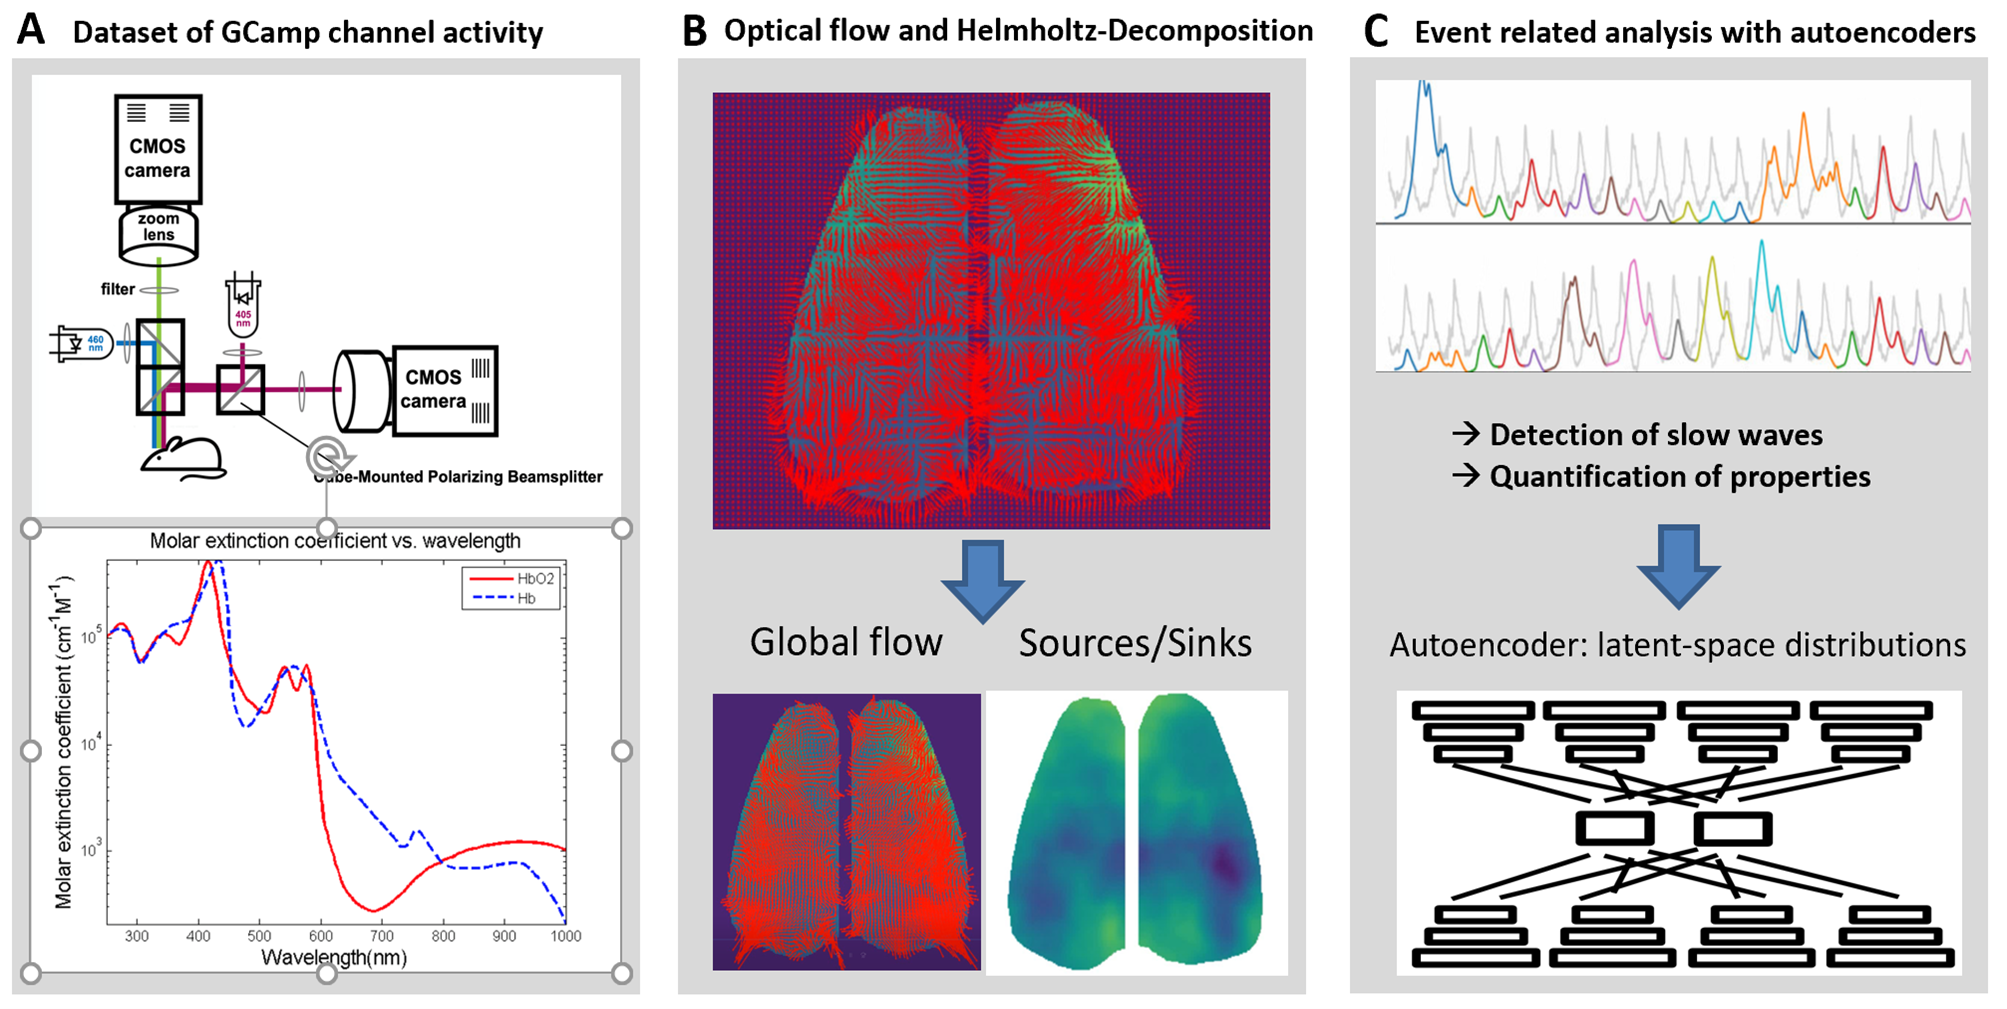
\includegraphics[width=\textwidth,height=\textheight,keepaspectratio]{Figures/outline_approach}
\decoRule
\caption[Outline of the approach]{Outline of the approach\\Panel A: Dataset of GCamp channel activity. The main dataset used to develop and evaluate the approach presented here includes recordings of GCamp fluorescence of transgenic mice. Recordings were acquired for different stages of anaesthesia ranging from 1.8\% isoflurane to 2.6\%. The sampling rate is 100Hz with a spatial resolution of 300x260px. GCamp flouroscence was recorded under illumination with light at 460nm. The hemodynamic fluorescence was recoded at 25Hz under illumination with light of 405nm wavelength. Polarization filters and beam splitters were used to acquire both signals at the same time. All depictions of Panel A were provided by Westmeyer Laboratory. All recordings were performed by Silviu Bodea at Westmeyer Laboratory at Technische Universität München. Panel B: Optical Flow and Helmholtz-Decompositon. The panel shows schematically how optical-flow can be estimated and decomposed into a global flow-field and a distribution of sources and sinks. This allows for the evaluation of pathways of neural signal transduction alongside the analysis of the spatial distribution of sources and sinks. Note that important features are derived from Optical Flow and Helmholtz-Decomposition but additional properties such as the correlation with the hemodynamic signal can be included in the analysis as well. Panel C: Event related analysis with autoencoders. The mean percentage change of the signal in time is used to identify individual slow-waves in a scale independent manner. This allows for the quantification of properties per-wave in an event-related design. Autoencoders are used to identify the relationship between properties of slow-waves including the experimental condition they stem from and aggregations of the results of Helmholtz Decomposition.}
\label{fig:outline_approach}
\end{figure}
Widefield flouroscence microscopy makes use of selective differences in the reflectance of light of a specific wavelength that results from conformational changes of ion channels in the neural membrane. The approach is challanged by the hemodynamic autoflourescence due to fluctuations in the blood oxygen level. The flouroscence of oxygenated and deoxigenated hemoglobin depends on the frequency of the light used for illumination. At a wavelength of 405nm the differences are marginal (Figure \ref{fig:outline_approach}:A). Hence the respective signal is referred to as GCaMP signal here. Nonetheless a hemodynamic error signal remains in the data. As it was found that high frequency oscillations relate to the bloodflow band stop filtering and smoothing were employed in preprocessing to reduce the effect of hemodynamics. The degree of temporal smoothing must be limited as fast spreading signals can otherwise not be detected. Components in the bandstop filtered signal that correspond to the heartbeat are absent in the result.\\
To assess the relationship between the GCaMP signal and the hemodynamic signal a second video was simultaneously recorded at 460nm using polarization filters and beamsplitters (Figure \ref{fig:outline_approach}:A). This hemodynamic signal was preprocessed in the same way as the GCaMP signal. High frequencies that include the range of the heartbeat are removed. It shows, that oscillations which are correlated to breathing are present in the signal. Removing this effect has proven difficult on the level of individual pixels especilly considering the requirement of a high temporal resolution that prohibits strong temporal smoothing. There is evidence which indicates that low amplitude oscillations in the GCaMP signal could at least partially include neural effects. \\
Arguments for respiration coupled neural effects can be summarized as follows. First the location of peak activity in the GCaMP signal and the hemodynamic signal can deviate. There is little coherence between the spatial distribution of both signals at peak activity. Second respiration coupled slow waves are not always perfectly phase locked with the hemodynamic signals but there can be a varying offset between the respiratory peaks in the GCaMP and the hemodynamic signal. While the amplitude of slow oscillations in the mean hemodynamic signal is relatively constant, the corresponding oscillations in the mean GCaMP signal can vary substantially - especially during deep anaesthesia. A possible explanation is that breathing coupled neural activity elicits neocortical slow waves in some cases while it is not sufficient in others. Finally, respiration coupled oscillations can be recorded using ECoG and have recently been proposed to represent an independant brain rythm that affects cortex \parencite{tort2018parallel}. As the question regarding the origin of breathing coupled oscillations in the GCaMP signal could not be finally answered no further efforts were taken towards a removal.\\
Slow waves are understood as extended periods of neural firing. ECoG data shows that several oscillations can occur during each event. The preprocessed df/f signal was further baseline corrected and used to distinguish events based on local minima. The minimal convex hull can be used for baseline correction. The df/f signal is (1) added to a parabola, (2) the convex hull is computed ("rubberband fit") and (3) subtracted from the signal. Because it is assumed that slow waves can include several oscillations events are not split at every local minimum. Instead a scanning procedure was implemented to determine local minima that define the $\text{start}$ and $\text{stop}$ positions. Beginning with the time of the first local minimum as $\text{start}$, subsequent local minima are evaluated recursively and defined as the $\text{stop}$ of the current event if the activity is sufficiently close to baseline. The latter condition holds if the value $f(\text{stop})$ is not larger then $f(\text{start}) + \epsilon$. Epsilon is expressed as the current height of the event i.e. the absolute difference between $f(\text{start})$ and the maximal value between $f(\text{start})$ and $f(\text{stop})$. The approach allows to split events of different magnitude without using a hard threshold.\\
\begin{figure}[!htb]
\centering
\includegraphics[width=\textwidth,height=\textheight,keepaspectratio]{Figures/diagram_pipeline}
\decoRule
\caption[The processing pipeline]{The processing pipeline}
\label{fig:diagram_pipeline}
\end{figure}
The indices that result from the splitting procedure are used to compute a contrast for each event seperately. The computation of the df/f signal per event has two advantages. First movements of the animal do not affect the whole contrast for the whole recording. If the animal moves slightly the mean image and the individual frames are misaligned. This leads to artifacts in the df/f signal. In an event related design this affects at worst single events. Similarly it allows to subtract the mean image after computing the background to improve the contrast as suggested by Celotto et al. \parencite{celotto2020analysis}. Second the mean image represents a biased proxy for an image of the brain where no GCaMP flouroscence occurs. In average slow wave activity is stronger in certain regions, hence the mean image is brighter. While this does not impose a problem for large amplitude events it is clearly visible as a spatial bias in the df/f signal of small amplitude events. If the contrast is computed for each event seperately this effect is reduced and local differences become visible.\\
In the last two steps of the pipeline Optical Flow and Helmholtz Decomposition are used to characterize the dynamics of the events and several features are aggregated and stored in a sparse dataset. This dataset contains information about the df/f signal, the distribution of sources and sinks as well as several aggregations of the vector fields of the flow component.
